\documentclass[a4paper]{article}

\usepackage[english]{babel}
\usepackage[utf8]{inputenc}
\usepackage{amsmath}
\usepackage{graphicx}
\usepackage[breaklinks]{hyperref}
\usepackage{caption}
\usepackage{listings}
\usepackage[round]{natbib}
\bibliographystyle{plainnat}


\title{
	Project 02 \\
	\bigskip
	\normalsize APSC 607 Fall 2017
}

\author{Seth Goodman}

\date{\today}


\begin{document}
\maketitle


%\begin{abstract}
%\end{abstract}

\section{Introduction}
\label{sec:introduction}

This project explores different numerical methods for calculating the definite integrals of functions. Each functions will be examined in the range between zero and two, using the Composite Trapezoidal Rule, Composite Midpoint Rule, Composite Simpson’s Rule, as well as an adaptive implementation of Simpson’s Rule. The behavior and characteristics of these methods will be reviewed by examining the effectiveness of the resulting value for the integral when using varying number of subintervals, \textbf{n}. For each \textbf{n}, the result will be evaluated with respect to the true integral value using defined tolerances thresholds. 

All computations are performed using MATLAB using the code accompanying this report (in a zip file). The following \textit{Methods} section will present the methods used in MATLAB to explore functions, as well as the outputs and results. The \textit{Results} section of this report contains the outputs for each function along with related observations and discussion. All figures and tables found in this report are available in the output subdirectory of the accompanying zip file. Additionally, all code and figures found in the zip file can be accessed via GitHub\footnote{\url{https://github.com/sgoodm/apsc607/tree/master/project_02}}.



\newpage
\section{Methods}
\label{sec:methods}

The two unique functions which will be explored in this project, Functions \textbf{A} and \textbf{B}, are defined by Equations \ref{eq:fa} and \ref{eq:fb}, respectively. 

\begin{equation}
f(x) = e^{2x} * sin(3x)
\label{eq:fa}
\end{equation}

\begin{equation}
f(x) = \frac{1}{x+4}
\label{eq:fb}
\end{equation}

To establish a baseline for error comparisons, the true value for the integral of each function is first calculated using built in MATLAB tools. The integral is calculated both using the symbolic toolkit function \textbf{int} as well as the numerical function \textbf{integral}. The resulting values can be seen in Table \ref{true_values}.

\bgroup
\def\arraystretch{1.5}
\begin{center}
	\centering
	\begin{tabular}{l|r|r}
	\textbf{Function} & \textbf{Symbolic} & \textbf{Numeric} \\
	\hline
	A & -14.2139771298625 & -14.2139771298625\\
	B & 0.405465108108164 & 0.405465108108164
	\end{tabular}
	\captionof{table}{True values of integrals between zero and two}
	\label{true_values}
\end{center}
\egroup

The true value for Functions A and B will be compared to the results of integration using the Trapezoidal, Midpoint, and Simpson's Rules for a range of subintervals. The range of subinterval values, \textbf{n}, will vary with each function and rule tested, in order to achieve accuracy within a tolerance of $1e^{-4}$ and $1e^{-8}$. 

The tolerance is defined as the absolute difference between the result of numerical integration at a given \textbf{n} value and the true value of the integral. An alternative approach for measuring tolerance is to compare the difference between the integral resulting from subsequent values of \textbf{n}. Both methods will effectively illustrate the performance of the different methods of numerical integration, but comparing to the true value provides a independent metric of accuracy, rather than one which is dependent on the step size between values of \textbf{n}. Since the accuracy tolerance will not be based on subsequent values of \textbf{n}, a sample of values for \textbf{n} can be used rather than the full range. This will drastically improve the performance of the MATLAB calculations without sacrificing noticeable detail from the results. Figure \ref{fig:sample_comparison} illustrates an example of the sampling points used for \textbf{n} ranging between 2 and 100,000. As a tradeoff for reduced computation time, the apparent value of \textbf{n} required to achieve a given tolerance can be inflated as seen in Table \ref{table:sample_comparison}. Sampling may not be ideal in all scenarios, but works well as an exploratory technique when the magnitude of the upper limit of the \textbf{n} values is unknown and the potential number of \textbf{n} values which need to be tested is very large.

\bgroup
\def\arraystretch{1.5}
\begin{center}
	\centering
	\begin{tabular}{l|r|r}
	\textbf{Tolerance} & \textbf{Full Range} & \textbf{Sample} \\
	\hline
	$1e^{-4}$ & 644 & 768\\
	$1e^{-8}$ & 64230 & 65536
	\end{tabular}
	\captionof{table}{Example \textbf{n} needed to reach tolerance by sampling \textbf{n} vs using full range}
	\label{table:sample_comparison}
\end{center}
\egroup

\begin{center}
	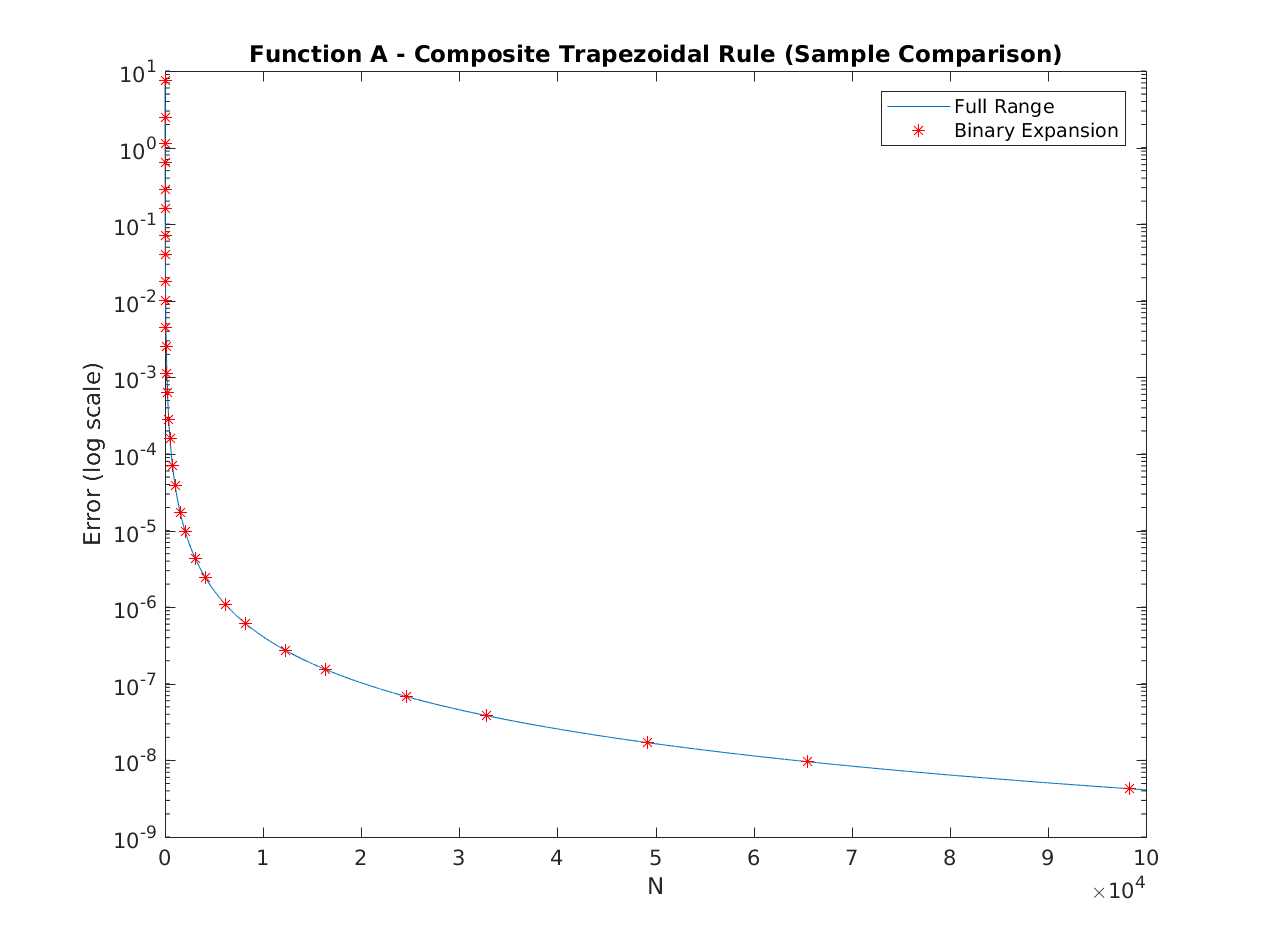
\includegraphics[width=1\textwidth]{../output/a_trapezoidal_sample_comparison.png}
	\captionof{figure}{Sample Comparison}
	\label{fig:sample_comparison}
\end{center}

The value of \textbf{n} required to reach the specified tolerance is dependent on the function itself as well as the error term associated with each rule. The error terms for the Trapezoidal, Midpoint, and Simpson's Rules are defined in Equation \ref{trap_err}, \ref{mid_err}, and \ref{sim_err} respectively \citep{burden2010}. As the Trapezoidal and Midpoint Rules have second order error terms, it is expected that they will require a greater value of \textbf{n} to produce results comparable to Simpson's Rule, which has a fourth order error term.

\begin{equation}
\frac{b-a}{6}h^2f^{''}(u)
\label{trap_err}
\end{equation}

\begin{equation}
\frac{b-a}{12}h^2f^{''}(u)
\label{mid_err}
\end{equation}

\begin{equation}
\frac{h^5}{90}f^{(4)}(\xi_j)
\label{sim_err}
\end{equation}

All values of \textbf{n} tested will be positive and even, as it is required for the Midpoint and Simpson's Rules. Although the Trapezoidal Rule can be used with odd intervals, using only even intervals will provide sufficient sample points for analysis. In order to test \textbf{n} over a sufficient range for the Trapezoidal and Midpoint Rules, a binary expansion will be used to generate values of \textbf{n} at which to sample the full range, rather than test at every possible step. Starting with two sub intervals ($n=2$), if every even sub interval value up to 100,000 was tested it would require 50,000 points. By incorporating a binary expansion based approach, a sample of only 20 different \textbf{n} values can generated which are capable of sufficiently demonstrating the behavior of the integration rules.

Due to the higher order error term, Simpson's Rule can reach the desired tolerance much quicker and a simple range of $2:2:nmax$ can be used. 

The functions implementing the Trapezoidal, Midpoint, and Simpson's Rules will be called over the range of values for \textbf{n} using the \textbf{arrayfun} function in MATLAB. This function accepts another function, defining our integration rule, and a vector, and simply repeatedly calls the specified value while iterating over the values in the vector. The call to \textbf{arrayfun} then return a vector (or set of vectors in this case) containing the results from each call to the integration function. A simplified example below show the \textbf{arrayfun} function being used to pass each \textbf{n} value in a vector called \textbf{nlist} to a trapezoidal function, returning a vector of the resulting output values.

\bigskip
\begin{lstlisting}[language=Matlab]
[int_vals] = arrayfun(@(n) trapezoidal(n), nlist);
\end{lstlisting}
\bigskip

 The resulting vector of integral values across varying \textbf{n} can compared with the true integral value generated earlier, to produce an error vector. The error vector is used to identify the value of \textbf{n} (and thus \textbf{h}) at which the integration rule produced results that were accurate within a desired tolerance. No \textbf{n} value needs to be specified for the adaptive approach because, as seen in Subsection \ref{method:adaptive}, this approach iteratively checks (within the function) that a specified tolerance has been reached before producing a single output rather than using a set \textbf{n} value to produce a set of output values.

The remainder of this section will introduce the three composite numerical integration approaches (Trapezoidal, Midpoint, and Simpson's) and the adaptive approach using Simpson's Rule.


\subsection{Composite Trapezoidal Rule}\label{method:trapezoidal}

\begin{center}

	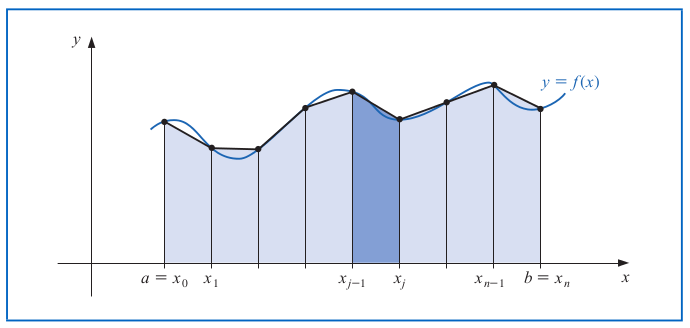
\includegraphics[width=1\textwidth]{../additional/trapezoidal_fig.png}
	\captionof{figure}{Trapezoidal Figure \citep{burden2010}}
	\label{trap_fig}
\end{center}


The Composite Trapezoidal Rule for $n$ intervals, as seen in Figure \ref{trap_fig}, can be defined by Equation \ref{trap_eq}, given $h=(b-a)/n$ and $x_j=a+jh$, for each $j=0,1,\dots,n$ \citep{burden2010}.

\begin{equation}
\int_{a}^b f(x) dx = \frac{h}{2} \Bigg[ f(a) + 2 \sum_{j=1}^{n-1} f(x_j) + f(b) \Bigg]
\label{trap_eq}
\end{equation}

In this equation, the integral of each individual subinterval is calculated simply as the area of a trapezoid:

\begin{equation}
area_{subinterval} = \frac{f(x_j) + f(x_{j+1})}{2}h
\end{equation}


\subsection{Composite Midpoint Rule}\label{method:midpoint}

\begin{center}
	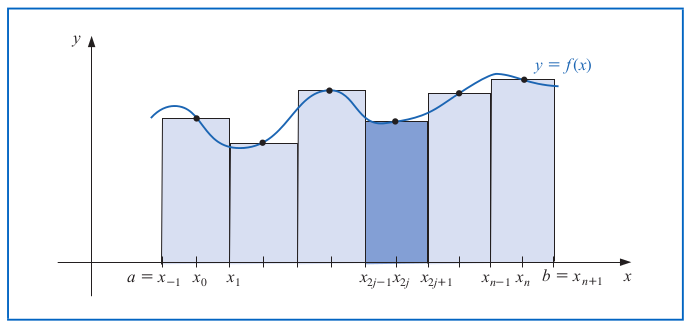
\includegraphics[width=1\textwidth]{../additional/midpoint_fig.png}
	\captionof{figure}{Midpoint Figure \citep{burden2010}}
	\label{mid_fig}
\end{center}

The Composite Midpoint Rule for $n+2$ intervals, as seen in Figure \ref{mid_fig}, can be defined by Equation \ref{mid_eq}, given $h=(b-a)/(n+2)$ and $x_j=a+(j+1)h$, for each $j=-1,0,\dots,n+1$ \citep{burden2010}.

\begin{equation}
\int_{a}^b f(x) dx = 2h \sum_{j=0}^{n/2}f(x_2j)
\label{mid_eq}
\end{equation}

The area for each subinterval is similar to the Trapezoidal Rule, but instead of calculated the area of a trapezoid, the midpoint of the subinterval is used to calculate the area of a rectangle:

\begin{equation}
area_{subinterval} = f(\frac{x_{2j-1}+x_{2j+1}}{2})h
\end{equation}

\subsection{Composite Simpson's Rule}\label{method:simpsons}

\begin{center}
	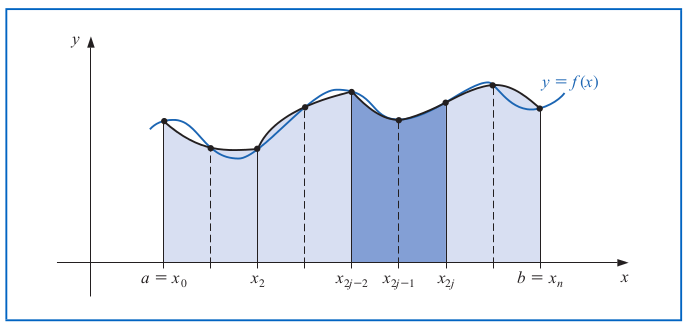
\includegraphics[width=1\textwidth]{../additional/simpsons_fig.png}
	\captionof{figure}{Simpson's Figure \citep{burden2010}}
	\label{sim_fig}
\end{center}

The Composite Simpson's Rule for $n$ intervals, as seen in Figure \ref{sim_fig}, can be defined by Equation \ref{sim_eq}, given $h=(b-a)/n$ and $x0_j=a+jh$, $x1_j=a+jh+h/2$, $x2_j=a+jh+h$,  for each $j=0,1,\dots,n-1$.
     
\begin{equation}
\int_{a}^b f(x) dx = \sum_{j=0}^{n-1} \Bigg[ \frac{h}{6} \big[ f(x0_j) + 4f(x1_j) + f(x2_j) \big] \Bigg]
\label{sim_eq}
\end{equation}



\subsection{Adaptive Simpson's Rule}\label{method:adaptive}

\bigskip
\begin{lstlisting}[language=Matlab]


integral_value = 0

subinterval_data = [
    {	
	    a = bound_min
	    b = bound_max
    }, 
    {...}, 
    ...
]

number_of_subintervals_remaining = 1


while number_of_subintervals_remaining > 0

	active_interval = simpsons(a,b)
	
	left_half = simpsons(a, (b-a)/2)
	right_hal = simpsons((b-a)/2, b)
	
	if active - (left_half+right_half) < tolerance
		
		tolerance reached
		integral_value += active_interval
		
	else
		save left half definition
		number_of_subintervals_remaining += 1
		subinterval_data.append({aleft, bleft}

		save right half definition		
		number_of_subintervals_remaining += 1
		subinterval_data.append({aleft, bleft}
		
		% next loop of while loop will process this right half
		% continuehalving and working down right most subinterval until tolerance reached
		% then work backwards towards the leftmost subinterval until all subinterval which make upthe original range have been processed		

\end{lstlisting}
\bigskip



\newpage
\section{Results}
\label{sec:results}

TEXT


Something about minimum error in footnote\footnote{See following link on MATLAB precision limitions (general limitations of floating point representations apply) https://www.mathworks.com/help/fixedpoint/ug/limitations-on-precision.html}.


\subsection{A}\label{results:a}

\begin{center}
	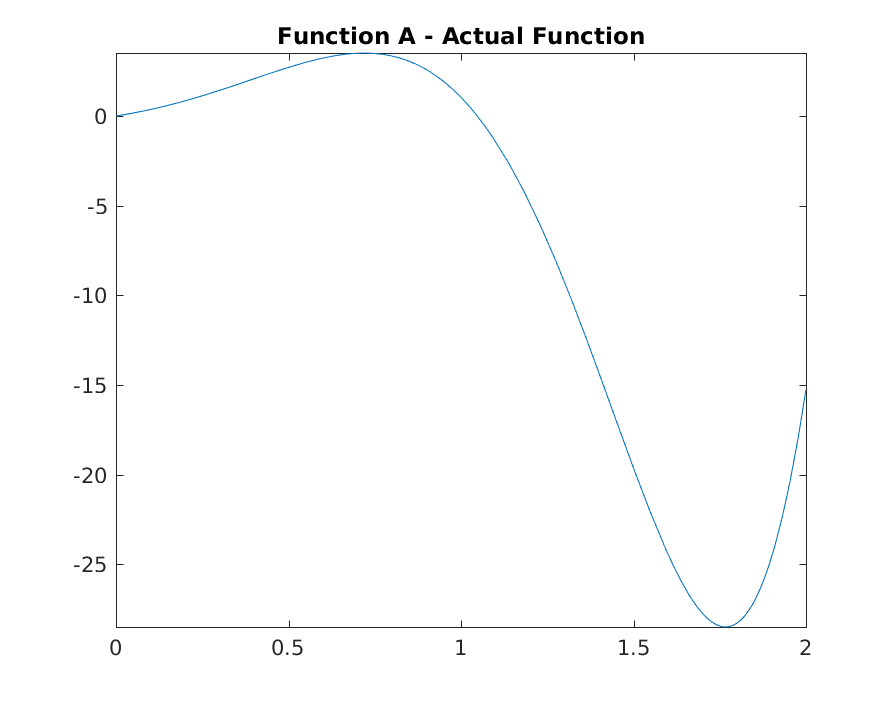
\includegraphics[width=1\textwidth]{../output/a_actual.png}
	\captionof{figure}{caption text a}
	\label{fig:a_act}
\end{center}

\begin{center}
	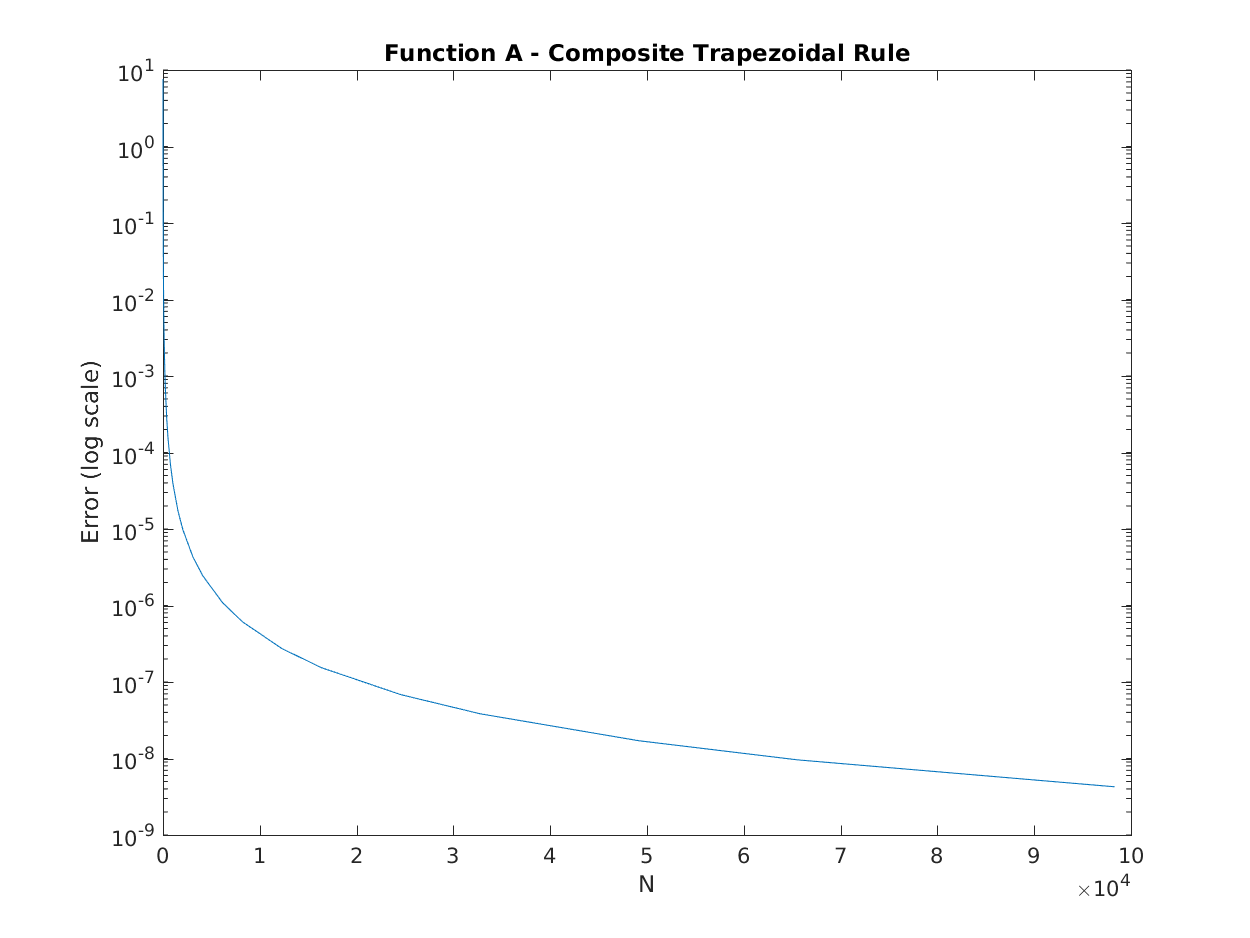
\includegraphics[width=1\textwidth]{../output/a_trapezoidal.png}
	\captionof{figure}{caption text a}
	\label{fig:a_trap}
\end{center}


\begin{center}
	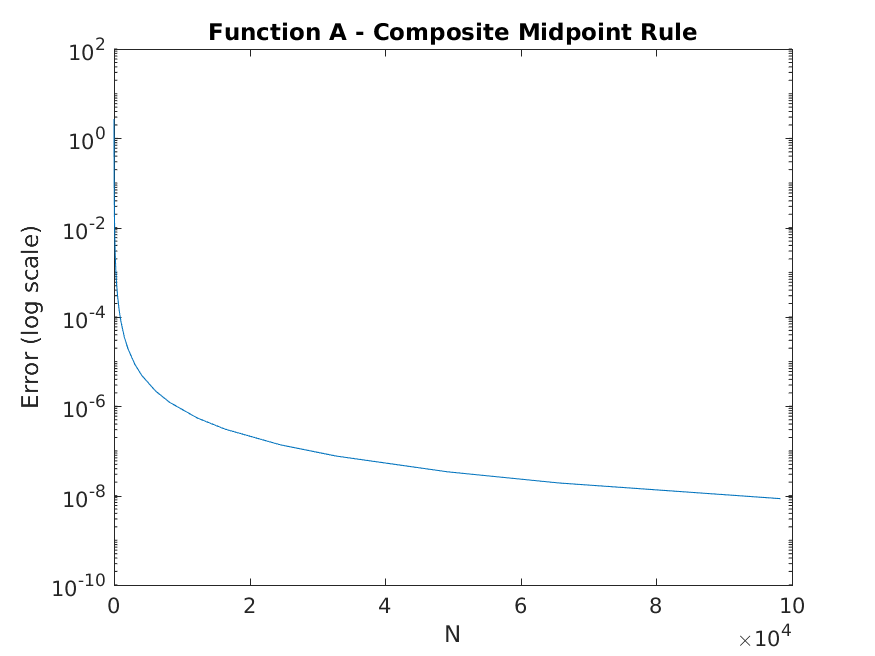
\includegraphics[width=1\textwidth]{../output/a_midpoint.png}
	\captionof{figure}{caption text a}
	\label{fig:a_mid}
\end{center}


\begin{center}
	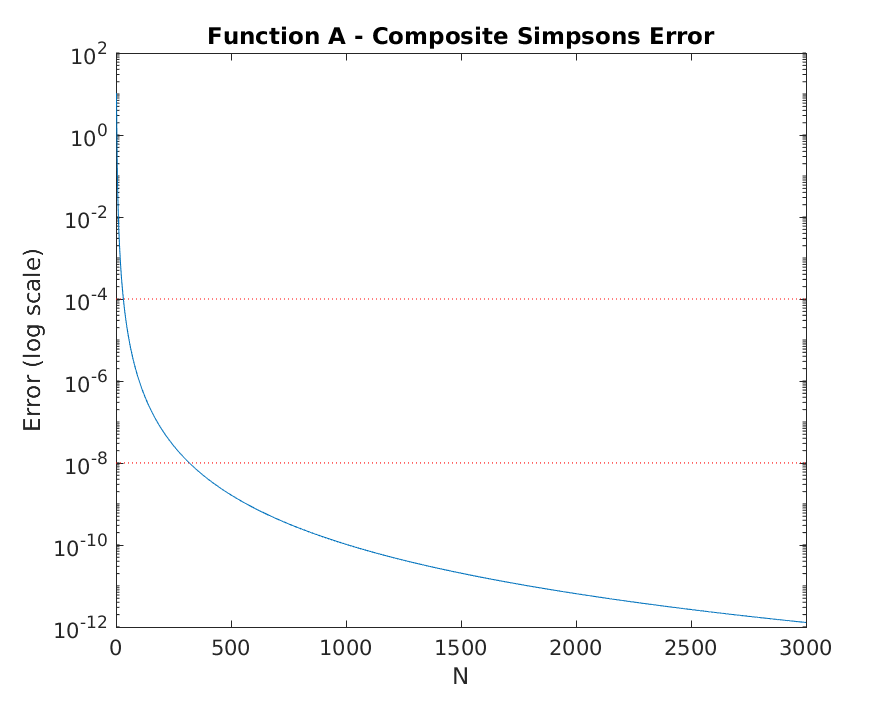
\includegraphics[width=1\textwidth]{../output/a_simpsons.png}
	\captionof{figure}{caption text a}
	\label{fig:a_sim}
\end{center}


\begin{center}
	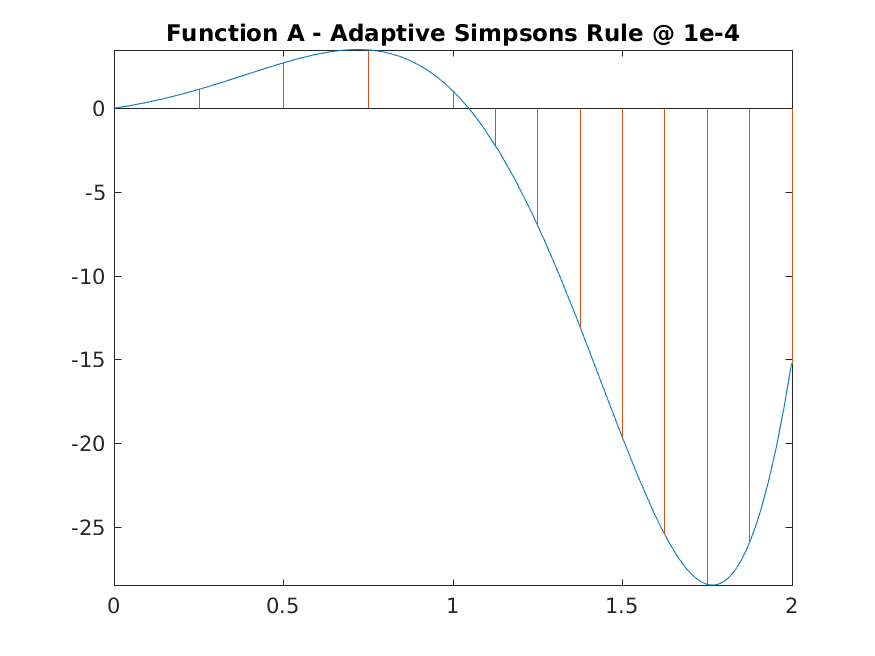
\includegraphics[width=1\textwidth]{../output/a_adaptive_simpsons_4.png}
	\captionof{figure}{caption text a}
	\label{fig:a_adap4}
\end{center}

\begin{center}
	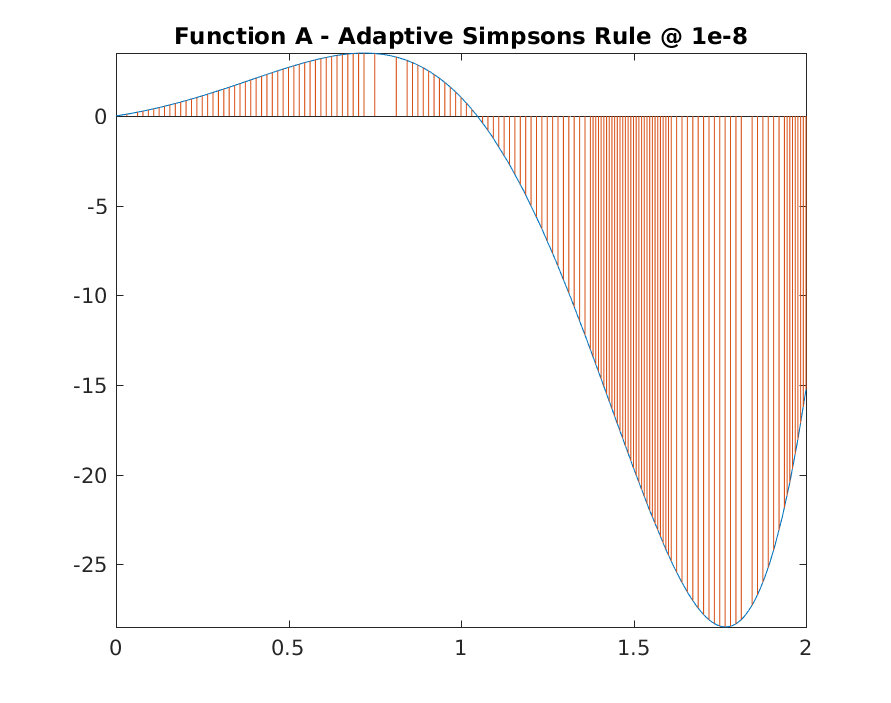
\includegraphics[width=1\textwidth]{../output/a_adaptive_simpsons_8.png}
	\captionof{figure}{caption text a}
	\label{fig:a_adap8}
\end{center}



\subsection{B}\label{results:b}

\begin{center}
	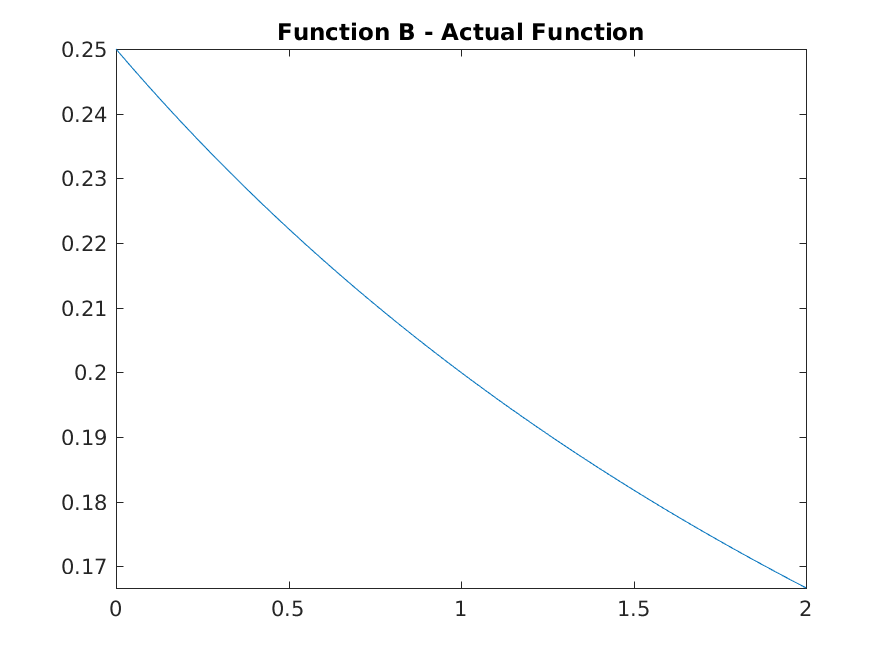
\includegraphics[width=1\textwidth]{../output/b_actual.png}
	\captionof{figure}{caption text a}
	\label{fig:b_act}
\end{center}

\begin{center}
	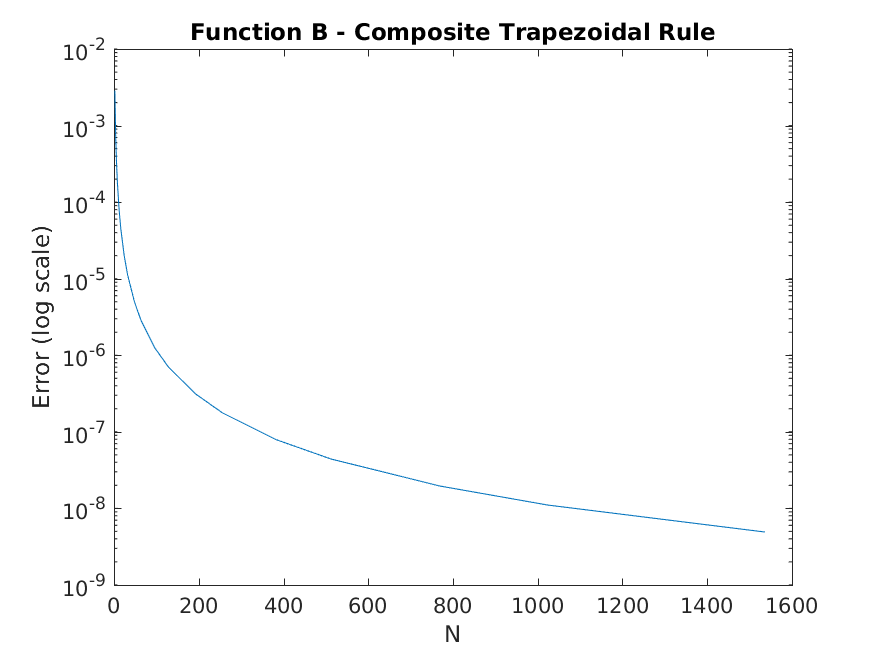
\includegraphics[width=1\textwidth]{../output/b_trapezoidal.png}
	\captionof{figure}{caption text a}
	\label{fig:b_trap}
\end{center}


\begin{center}
	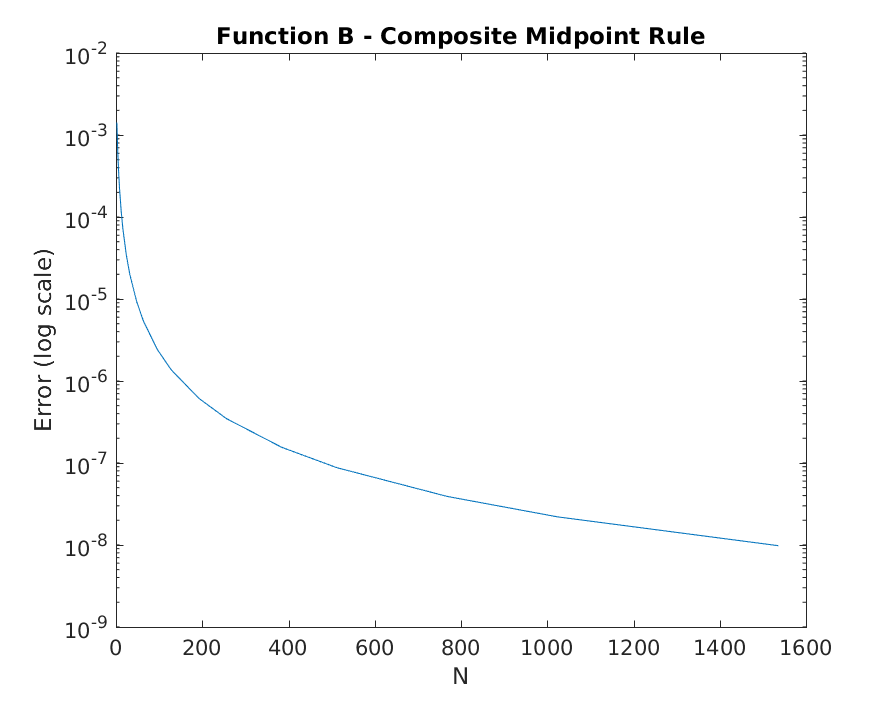
\includegraphics[width=1\textwidth]{../output/b_midpoint.png}
	\captionof{figure}{caption text a}
	\label{fig:b_mid}
\end{center}


\begin{center}
	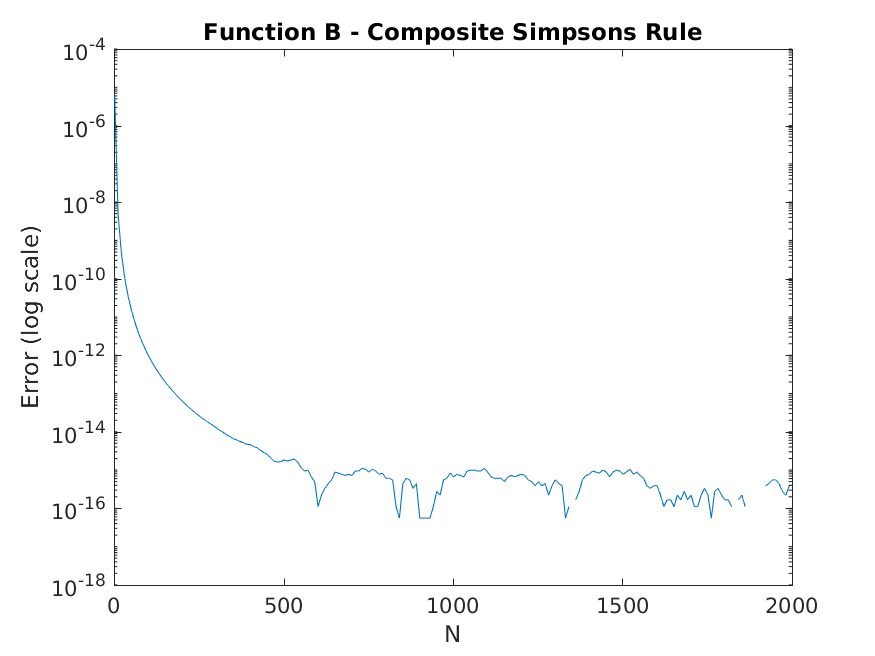
\includegraphics[width=1\textwidth]{../output/b_simpsons.png}
	\captionof{figure}{caption text a}
	\label{fig:b_sim}
\end{center}


\begin{center}
	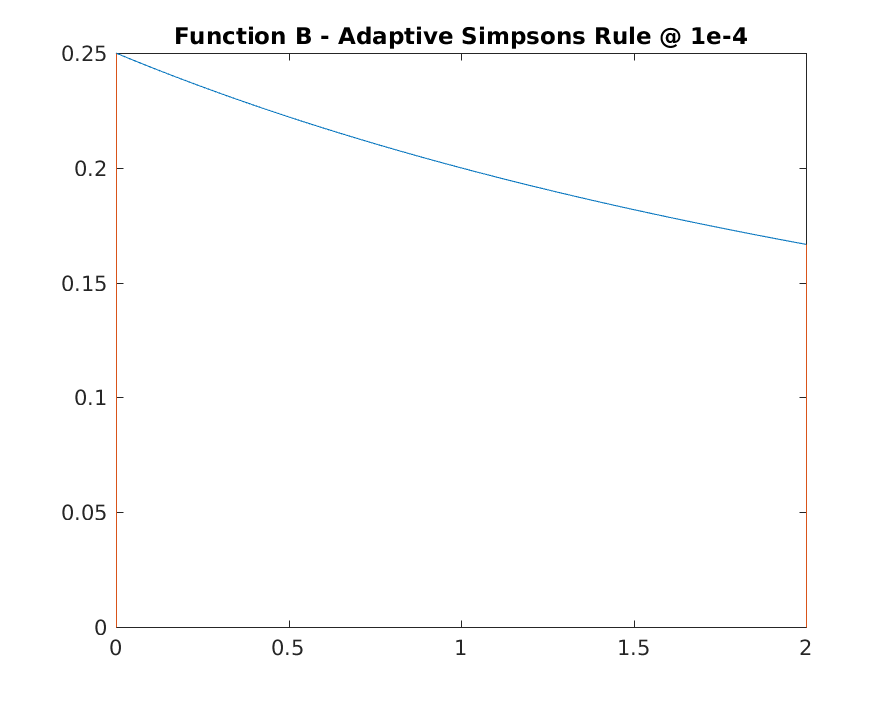
\includegraphics[width=1\textwidth]{../output/b_adaptive_simpsons_4.png}
	\captionof{figure}{caption text a}
	\label{fig:b_adap4}
\end{center}

\begin{center}
	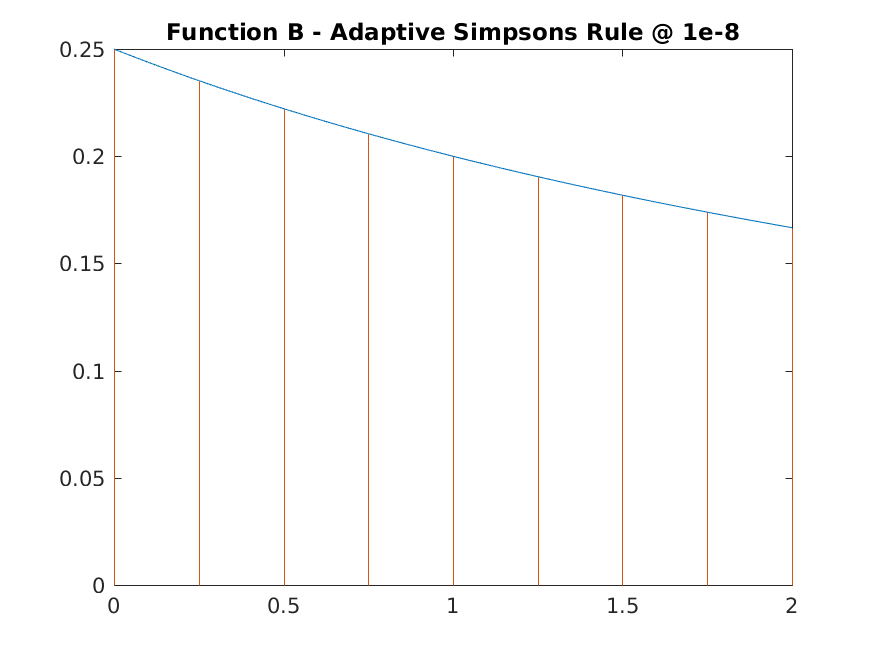
\includegraphics[width=1\textwidth]{../output/b_adaptive_simpsons_8.png}
	\captionof{figure}{caption text a}
	\label{fig:b_adap8}
\end{center}






\subsection{Expanded Range}\label{results:expanded}


 integration over an expanded range and the potential utility of adaptive approaches in such a scenario

\begin{center}
	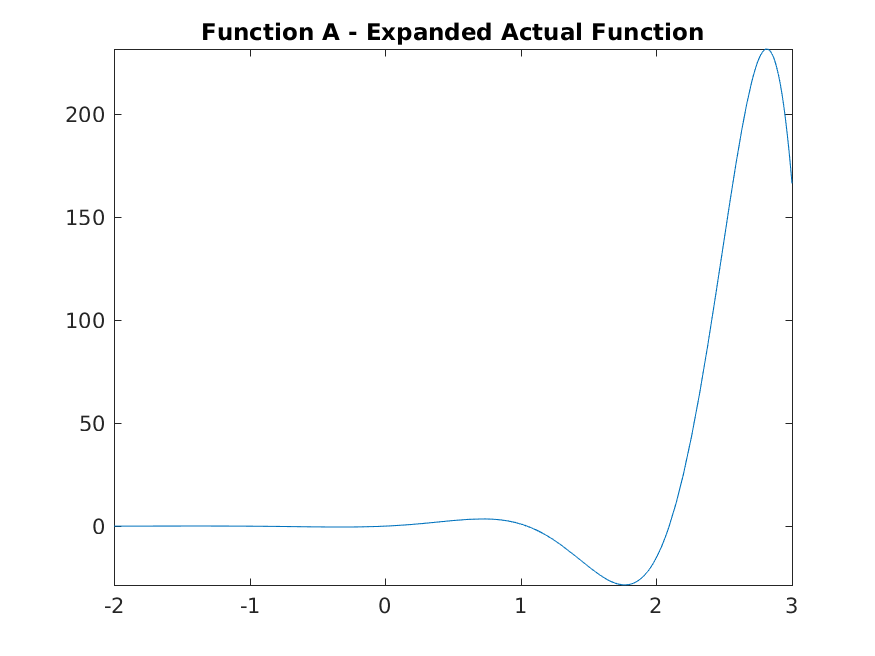
\includegraphics[width=1\textwidth]{../output/a_expanded_actual.png}
	\captionof{figure}{caption text a}
	\label{fig:a_ex}
\end{center}


\begin{center}
	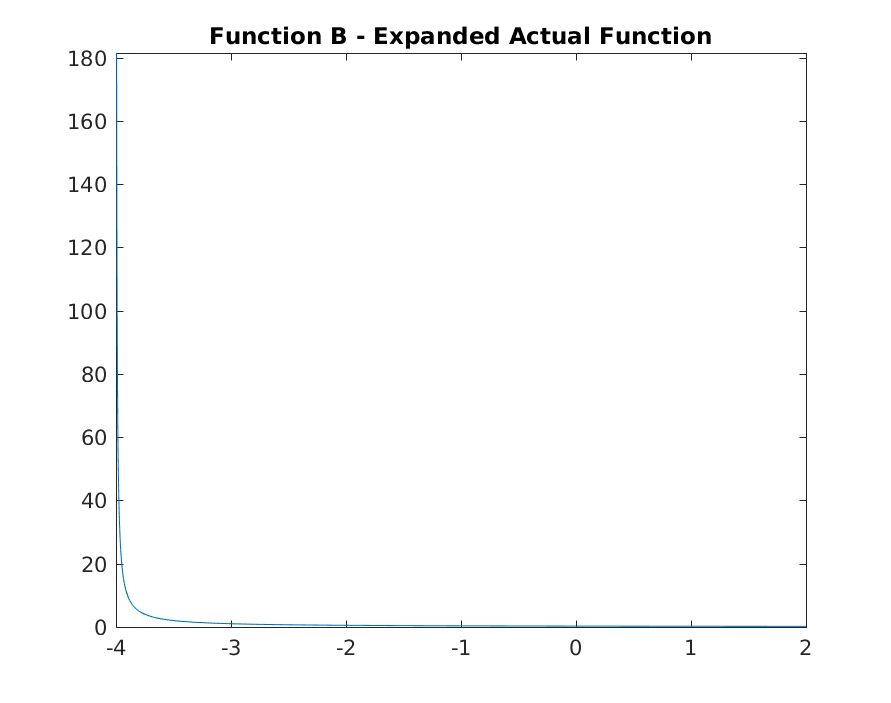
\includegraphics[width=1\textwidth]{../output/b_expanded_actual.png}
	\captionof{figure}{caption text a}
	\label{fig:b_ex}
\end{center}











\newpage

\bibliography{report}


\end{document}
